\sezione{8}{Normale multivariata e distanza di Mahalanobis}{31, 40–43}

Qui tutti i pezzi della sezione 7 si incastrano: la campana della sezione 6 viene generalizzata a $d$ feature.

\subsection{Notazione}
\begin{itemize}
  \item $\x_i$: pattern $i$-esimo del training set (\textbf{vettore}, indice in basso);
  \item $x_i^j$: componente $j$-esima del pattern $i$-esimo (\textbf{scalare}, indice in alto). Attenzione: l'apice è un indice, non una potenza.
  \item I vettori sono \emph{colonne}; l'apice $\mathsf{t}$ li trasforma in righe.
\end{itemize}

\subsection{La formula}
\begin{formulat}{Densità multinormale ($d>1$)}
$\displaystyle p(\x)=\frac{1}{(2\pi)^{d/2}\,|\SSigma|^{1/2}}\;\exp\!\left[-\frac12\,(\x-\mmu)\T\,\SSigma^{-1}\,(\x-\mmu)\right]$
\end{formulat}
dove $\mmu=[\mu^1,\dots,\mu^d]\T$ è il \key{vettore medio} e $\SSigma=[\sigma^{ij}]$ la \key{matrice di covarianza} $d\times d$.

\begin{intuizione}[Confronto pezzo per pezzo con il caso 1D]
\begin{center}
\begin{tabular}{lcc}
\toprule
& \textbf{1D} & \textbf{$d$ dimensioni}\\
\midrule
centro & $\mu$ & $\mmu$\\
«larghezza» & $\sigma^2$ & $\SSigma$\\
distanza al quadrato & $(x-\mu)^2/\sigma^2$ & $(\x-\mmu)\T\SSigma^{-1}(\x-\mmu)$\\
normalizzazione & $\sigma\sqrt{2\pi}$ & $(2\pi)^{d/2}|\SSigma|^{1/2}$\\
\bottomrule
\end{tabular}
\end{center}
Dividere per $\sigma^2$ diventa moltiplicare per $\SSigma^{-1}$; la $\sigma$ della normalizzazione diventa $|\SSigma|^{1/2}$, il «volume» della nuvola.
\end{intuizione}
\begin{tecnica}[Le dimensioni tornano]
$(\x-\mmu)\T$ è $1\times d$, $\SSigma^{-1}$ è $d\times d$, $(\x-\mmu)$ è $d\times1$: il prodotto è $1\times1$, cioè un \textbf{numero}. L'esponente è uno scalare, come deve essere.
\end{tecnica}

\subsection{Quanti parametri?}
$\SSigma$ è simmetrica, quindi basta conoscere la diagonale e metà degli elementi restanti: $\dfrac{d(d+1)}{2}$ parametri, più i $d$ della media.
\begin{center}
\rowcolors{2}{chiaro}{white}
\begin{tabular}{cccc}
\rowcolor{navy}\thd{$d$} & \thd{media} & \thd{covarianza piena} & \thd{covarianza diagonale}\\
2 & 2 & 3 & 2\\
10 & 10 & 55 & 10\\
100 & 100 & 5050 & 100\\
\end{tabular}
\end{center}
Con molte feature la covarianza piena richiede moltissimi dati per essere stimata bene (e per essere invertibile, sezione 7): è uno dei motivi del successo del Naive Bayes.

\subsection{Varianze e covarianze}
Gli elementi diagonali $\sigma^{ii}=(\sigma^i)^2$ sono le varianze delle singole feature; quelli fuori diagonale le covarianze:
\begin{itemize}
  \item $x^i,x^j$ statisticamente indipendenti $\Rightarrow\sigma^{ij}=0$;
  \item correlate positivamente $\Rightarrow\sigma^{ij}>0$ (quando cresce una cresce l'altra);
  \item correlate negativamente $\Rightarrow\sigma^{ij}<0$.
\end{itemize}
\begin{attenzione}[L'implicazione vale in un solo verso]
Indipendenza $\Rightarrow$ covarianza nulla, ma in generale \textbf{non} il contrario: la covarianza misura solo legami \emph{lineari} ($x$ e $x^2$ con $x$ simmetrica attorno a 0 hanno covarianza nulla ma sono dipendenti). Per la gaussiana multivariata, invece, covarianza nulla e indipendenza coincidono.
\end{attenzione}

\subsection{La forma: ellissi a densità costante}
Per $d=2$ le curve di livello della densità sono \textbf{ellissi} concentriche: i luoghi dei punti a densità costante.
\fig[.98\linewidth]{multinormali.pdf}
\didascalia{Stessa media, tre covarianze diverse. In arancione gli assi dell'ellisse, paralleli agli autovettori di $\SSigma$.}
\begin{tecnica}[Chi controlla cosa (slide 41–42)]
\begin{itemize}
  \item $\mmu=[\mu^1,\mu^2]$: posizione del \textbf{centro};
  \item $\sigma^{11},\sigma^{22}$: \textbf{allungamento} lungo i due assi;
  \item $\sigma^{12}=\sigma^{21}$: \textbf{rotazione} dell'ellisse rispetto agli assi cartesiani;
  \item gli assi dell'ellisse sono paralleli agli \textbf{autovettori} di $\SSigma$; le varianze lungo gli assi principali sono gli \textbf{autovalori}.
\end{itemize}
\end{tecnica}

\subsection{Covarianza diagonale e Naive Bayes}
Se $\sigma^{12}=0$ (matrice diagonale) gli assi dell'ellisse sono paralleli agli assi cartesiani e la multinormale si spezza in un \textbf{prodotto di $d$ normali 1D}:
\begin{formulat}{Covarianza diagonale}
$\displaystyle p(\x)=\prod_{j=1}^{d}\frac{1}{\sigma^j\sqrt{2\pi}}\exp\!\left[-\frac{(x^j-\mu^j)^2}{2(\sigma^j)^2}\right]$
\end{formulat}
\begin{mlbox}[Naive Bayes]
Il classificatore \textbf{Naive Bayes} assume che le feature siano indipendenti \emph{data la classe}: $p(\x|w_i)=\prod_j p(x^j|w_i)$. Con gaussiane è esattamente il caso diagonale: $2d$ parametri per classe invece di $d+d(d+1)/2$, nessuna matrice da invertire, stime stabili anche con pochi dati. L'ipotesi è quasi sempre falsa («naive», ingenua), eppure funziona bene su molti dataset, in particolare per la classificazione di testi: per questo è tra i classificatori più popolari.
\end{mlbox}

\subsection{La distanza di Mahalanobis}
\begin{formulat}{Distanza di Mahalanobis}
$\displaystyle r^2=(\x-\mmu)\T\,\SSigma^{-1}\,(\x-\mmu)\qquad\Longrightarrow\qquad p(\x)=\frac{1}{(2\pi)^{d/2}|\SSigma|^{1/2}}\,e^{-r^2/2}$
\end{formulat}
\begin{intuizione}
La densità dipende da $\x$ solo attraverso $r$: le ellissi a densità costante sono esattamente i luoghi a \textbf{distanza di Mahalanobis costante} ($r=1,2,3,\dots$). È la generalizzazione di «quante $\sigma$ dista dal centro?». Rispetto alla distanza euclidea, Mahalanobis \textbf{pesa} ogni direzione in base a quanto i dati variano lungo di essa e tiene conto della \textbf{correlazione}: un passo lungo la direzione in cui la nuvola è allungata conta poco, uno nella direzione stretta conta molto.
\end{intuizione}
\begin{minipage}[c]{.5\linewidth}
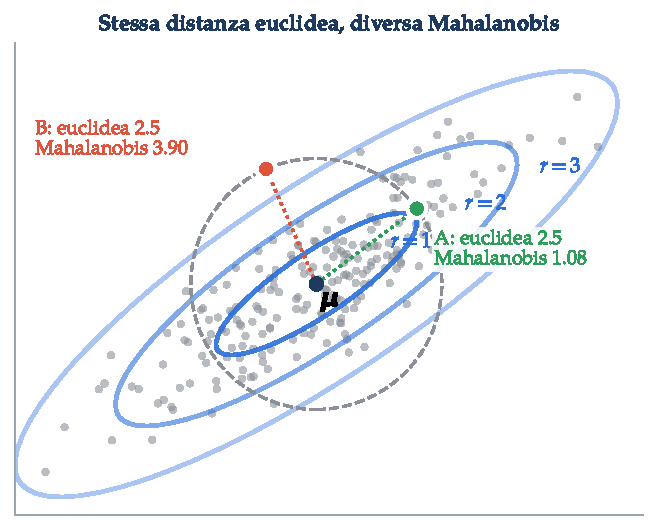
\includegraphics[width=\linewidth]{figs/mahalanobis.pdf}
\end{minipage}\hfill
\begin{minipage}[c]{.47\linewidth}\raggedright
\begin{esempio}[Stessa distanza euclidea]
I punti A e B distano entrambi 2.5 dal centro (cerchio tratteggiato), ma:
\begin{itemize}
  \item A sta lungo l'asse lungo della nuvola: $r\approx1.08$, è un punto \emph{tipico};
  \item B va «contro» la correlazione: $r\approx3.90$, è quasi un \emph{outlier}.
\end{itemize}
La distanza euclidea non vede la differenza; Mahalanobis sì.
\end{esempio}
\end{minipage}

\begin{tecnica}[Casi particolari]
\begin{itemize}
  \item $\SSigma=I$: $r^2=\|\x-\mmu\|^2$, Mahalanobis \textbf{coincide} con l'euclidea.
  \item $\SSigma$ diagonale: $r^2=\sum_j (x^j-\mu^j)^2/(\sigma^j)^2$, euclidea sulle feature \emph{standardizzate}.
  \item Se $\x$ è davvero gaussiano, $r^2$ segue una distribuzione $\chi^2$ con $d$ gradi di libertà: utile per riconoscere gli outlier.
\end{itemize}
\end{tecnica}
\begin{mlbox}
Mahalanobis si usa al posto dell'euclidea in k-NN e clustering quando le feature hanno scale diverse o sono correlate, e nel rilevamento di anomalie. Standardizzare le feature (z-score) prima di un k-NN è la versione «diagonale» della stessa idea.
\end{mlbox}

\begin{appunti}{— Sezione 8}
\pag{31} Pedice = pattern, apice = componente. $p(\x)=\frac{1}{(2\pi)^{d/2}|\SSigma|^{1/2}}\exp[-\frac12(\x-\mmu)\T\SSigma^{-1}(\x-\mmu)]$. Analogia 1D: $\sigma^2\to\SSigma$, $1/\sigma^2\to\SSigma^{-1}$, $\sigma\to|\SSigma|^{1/2}$. L'esponente è uno scalare.
\pag{40} Colonne, $\mathsf{t}$ = riga. Parametri di $\SSigma$: $d(d+1)/2$ (+ $d$ per $\mmu$). $\sigma^{ii}$ varianze; $\sigma^{ij}$ covarianze. Indipendenza $\Rightarrow\sigma^{ij}=0$ (il contrario vale per la gaussiana, non in generale).
\pag{41} $d=2$: ellissi = densità costante. $\mmu$ = centro; $\sigma^{11},\sigma^{22}$ = allungamento.
\pag{42} $\sigma^{12}$ = rotazione. $=0$: assi paralleli, prodotto di $d$ normali 1D = \textbf{Naive Bayes} ($2d$ parametri). Assi ∥ autovettori; varianze = autovalori. Naive Bayes funziona bene anche se l'ipotesi è falsa.
\pag{43} $r^2=(\x-\mmu)\T\SSigma^{-1}(\x-\mmu)$: le ellissi sono $r$ costante. Pesa per varianza e correlazione. $\SSigma=I$ → euclidea. Esempio: stessa euclidea 2.5, Mahalanobis 1.08 vs 3.90.
\end{appunti}
